
\hypertarget{menu_windows}{}
\section{Window}
\index{windows menu}

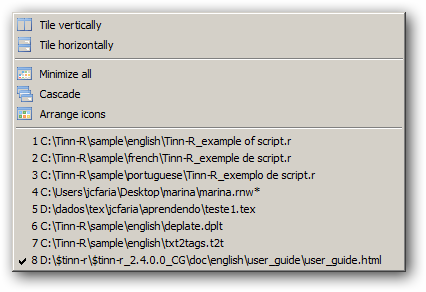
\includegraphics[scale=0.50]{./res/menu_window.png}\\

\begin{scriptsize}\begin{tabularx}{\textwidth}{>{\hsize=0.3\hsize}X>{\hsize=0.7\hsize}X}\\
    \hline
    \textbf{Option} & \textbf{Description} \\
    \hline
    Tile vertically & Shows two views of the same file tiled vertically, to the left and right. Each can be scrolled independently \\
    Tile horizontally & Shows two views of the same file tiled horizontally, one above the other. Each can be scrolled independently \\
    Minimize all & Minimizes all windows (editor) \\
    Cascade & The windows cascade from the upper left to the lower right of the workspace \\
    Arrange icons & Windows are tiled horizontally, but the active document comes on top. You may also drag your document tabs to the order you prefer and then tile them horizontally \\
    Files opened & If many files are opened, a dialog will be open to select a file \\
    \hline
  \end{tabularx}\end{scriptsize}
